%% ****** Start of file aiptemplate.tex ****** %
%%
%%   This file is part of the files in the distribution of AIP substyles for REVTeX4.
%%   Version 4.1 of 9 October 2009.
%%
%
% This is a template for producing documents for use with 
% the REVTEX 4.1 document class and the AIP substyles.
% 
% Copy this file to another name and then work on that file.
% That way, you always have this original template file to use.

%\documentclass[aip,reprint]{revtex4-1}
\documentclass[%
 aip,
%jmp,%
%bmf,%
%sd,%
rsi,%
 amsmath,amssymb,
%preprint,%
 reprint,%
%author-year,%
%author-numerical,%
]{revtex4-1}

\usepackage{graphicx}
\usepackage{float}
\usepackage{caption}
\usepackage{subcaption}

\draft % marks overfull lines with a black rule on the right

\begin{document}

% Use the \preprint command to place your local institutional report number 
% on the title page in preprint mode.
% Multiple \preprint commands are allowed.
%\preprint{}

\title{Report on current progress on two-species case: \\
competition-colonization trade-off and heteromyopia in 1D-, 2D- and 3D-spaces} %Title of paper

% repeat the \author .. \affiliation  etc. as needed
% \email, \thanks, \homepage, \altaffiliation all apply to the current author.
% Explanatory text should go in the []'s, 
% actual e-mail address or url should go in the {}'s for \email and \homepage.
% Please use the appropriate macro for the type of information

% \affiliation command applies to all authors since the last \affiliation command. 
% The \affiliation command should follow the other information.

\author{Alexey Nikitin}
\email[]{nikitin@cs.msu.ru}
%\homepage[]{Your web packagese}
%\thanks{}
\altaffiliation{National Research University Higher School of Economics, Faculty of Computer Science}
\affiliation{Lomonosov Moscow State University, Faculty of Computational Mathematics and Cybernetics}

\author{Anton Savostianov}
\email{a.s.savostyanov@gmail.com}
\affiliation{National Research University Higher School of Economics, Faculty of Computer Science}



% Collaboration name, if desired (requires use of superscriptaddress option in \documentclass). 
% \noaffiliation is required (may also be used with the \author command).
%\collaboration{}
%\noaffiliation

\date{\today}

\begin{abstract}
% insert abstract here
    Here we provide the report on the study of dimensionality effects on widely known coexistence mechanisms \emph{competition-colonization trade-off} and \emph{heteromyopia}. As usual we cover general problem statement, describe aforementioned mechanisms towards model's parameter space and show results obtained by developed numerical method. Background on the arising system of non-linear integral equations and numerical method's dimensional heuristics are provided in appendixes.
\end{abstract}

\pacs{}% insert suggested PACS numbers in braces on next line

\maketitle %\maketitle must follow title, authors, abstract and \pacs

%\begin{quotation}
%Hello!
%\end{quotation}

% Body of paper goes here. Use proper sectioning commands. 
% References should be done using the \cite, \ref, and \label commands
\section{Problem statement}
\label{sec:PrSt}
Assume that we are working with the basic model proposed in [Dieckmann, Law 2000] with following delimitations:
\begin{itemize}
    \item the population in the scope of the study consists of two species; in words, \(i, j, k = 1, 2\); 
    \item no restrictions considered for exogeniuos death rates, thus \( d_1 \ne 0 \), \( d_2 \ne 0 \);
    \item effects of kernel variation are not beyond the scope of the current research; \( m_i(\vec{\xi}) \) and \(w_{ij}(\vec{\xi})\) are distributed normally with zero mathematical expectation;
    \item in order to get numerical heuristics dispersal and competition kernels are supposed to be radially symmetric (s.t. \(f(\vec{\xi})=f(\lVert \vec{\xi} \rVert_2)\), which, we hope, can be treated as biologically reasonable assumption; 
    \item as we show in Appendix \ref{sec:appB}, previous bullet implies radial symmetry for all arising functions, in particular, for second moments \(C_{ij}(\xi) \);
    \item model supposed to be stationary, s.t. all movement events are realized through birth.
\end{itemize}
Here we put integro-differential equations arising in our model after
applying parametric closure:
\begin{multline*}
T_{ijk}(\xi,\xi') = \frac{\alpha}{2}\left(\frac{C_{ij}(\xi)C_{ik}(\xi')}{N_{i}}+\frac{C_{ij}(\xi)C_{jk}(\xi'-\xi)}{N_{j}}+\right.\\
  \left.+\frac{C_{ik}(\xi')C_{jk}(\xi'-\xi)}{N_{k}}-1\right)+(1-\alpha)\frac{C_{ij}(\xi)C_{ik}(\xi')}{N_{i}}
\end{multline*}
in system's dynamic equations:
\[
\frac{d}{dt}N_{i}=(b_{i}-d_{i})N_{i}-\sum_{j}\int_{\mathbb{R}^{n}}w_{ij}(\xi)C_{ij}(\xi)d\xi
\]
\begin{multline*}
\frac{d}{dt}C_{ij}(\xi)= \delta_{ij}m_{i}(-\xi)N_{i}+\int_{\mathbb{\mathbb{R}}^{n}}m_{i}(\xi')C_{ij}(\xi+\xi')d\xi'-\\-d_{i}C_{ij}(\xi)-\sum_{k}\int_{\mathbb{\mathbb{R}}^{n}}w_{ik}(\xi')T_{ijk}(\xi,\xi')d\xi-w_{ij}(\xi)C_{ij}(\xi)+\\+\langle i,j,\xi\to j,i,-\xi\rangle
\end{multline*}
We propose denotations such as $[f*g](\xi)=\int_{\mathbb{\mathbb{R}}^{n}}f(\xi')g(\xi'+\xi)d\xi'$
as classic \emph{convolution }and $y_{ij}=\int_{\mathbb{\mathbb{R}}^{n}}w_{ij}(\xi')C_{ij}(\xi')d\xi'$.
Also we use normalized moments $C_{ij}=\frac{C_{ij}}{N_{i}N_{j}}$
and $T_{ijk}=\frac{T_{ijk}}{N_{i}N_{j}N_{k}}$ and centralized $D_{ij}(\xi)=C_{ij}(\xi)-1$.
\par
As we stated earlier, \( i, j, k=1,2\). We study only physically understandable cases of \( n= 1, 2, 3 \). As proposed in [Law et al. 2003] we use chosen closure with 
\(
    \alpha=\frac 2 5
    \).

We study the distribution of the population in equilibium state, s.t.
\[
    \forall i,j: \; \frac{\partial N_i(t)}{\partial t}=0, \;\; \frac{\partial C_{ij}(\vec{\xi}, t)}{\partial t}=0
\]
    
\section{Mechanisms of co-existence}

\subsection{Competition-colonization trade-off}

Here we provide some more accurate illustrations for the competition-colonization trade-off which is a widely known mechanism of coexistence; the general rule is that more competitive species can coexist with better dispersed ones. In our study we have found it in $\left[\sigma_{m2};\;d'_{12}\right]$ parameter space.

We focus our research on effects of dimensionality for the described mechanism. Figures \ref{fig:cctod1}, \ref{fig:cctod2} and \ref{fig:cctod3} are devoted to $\mathbb{R}^1$, $\mathbb{R}^2$ and $\mathbb{R}^3$ respectively. We propose new improved method with fewer mistakes for two-dimensional
case and utterly new method for three-dimensional case. For each case we put two subfigures: surfaces of species densities for each pair \( (\sigma^m_2; d'_{12}) \) and areas in the parameter space that support co-existence or existence of only one species which is denoted by its number on the picture.

We stress out following things regarding obtained results and its further analysis:

\begin{figure*}
\centering
\begin{subfigure}{.5\textwidth}
  \centering
  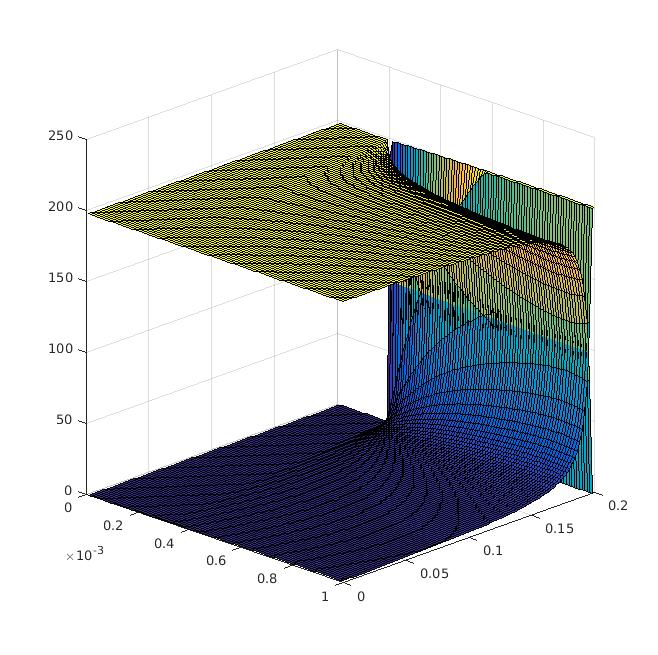
\includegraphics[width=.95\linewidth]{N1N2cctoD1.jpg}
  \caption{Surfaces of first moment \(N_1\) and \(N_2\) in described parameter space}
  \label{fig:cctod1:sub1}
\end{subfigure}%
\begin{subfigure}{.5\textwidth}
  \centering
  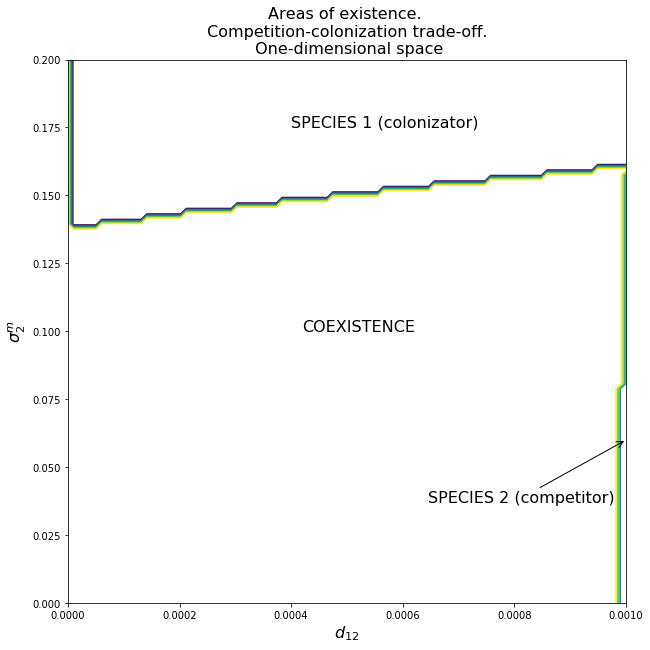
\includegraphics[width=.95\linewidth]{arccto08d1.png}
  \caption{Areas of coexistence in described parameter space} 
  \label{fig:cctod1:sub2}
\end{subfigure}
\caption{Realization of Competition-Colonization Trade-Off mechanisms in $\sigma^m_2$ and $d'_{12}$ parameter space in case of \emph{one-dimensional habitat}. Other parameters are chosen as follows:  $b_{1}=b_{2}=0.4
		, d_{1}=d_{2}=0.2
		, d'_{11}=d'_{22}=d'_{21}=0.001,
		\sigma_{1}^{m}=0.04
            , \sigma_{11}^{w}=\sigma_{12}^{w}=\sigma_{21}^{w}=\sigma_{22}^{w}=0.04$}
\label{fig:cctod1}
\end{figure*}

\begin{figure*}
\centering
\begin{subfigure}{.5\textwidth}
  \centering
  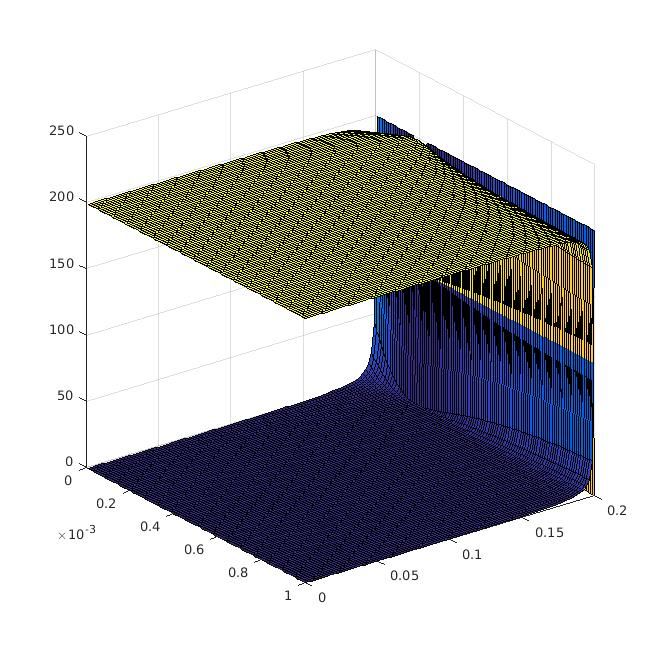
\includegraphics[width=.95\linewidth]{N1N2cctoD2.jpg}
  \caption{Surfaces of first moment \(N_1\) and \(N_2\) in described parameter space}
  \label{fig:cctod2:sub1}
\end{subfigure}%
\begin{subfigure}{.5\textwidth}
  \centering
  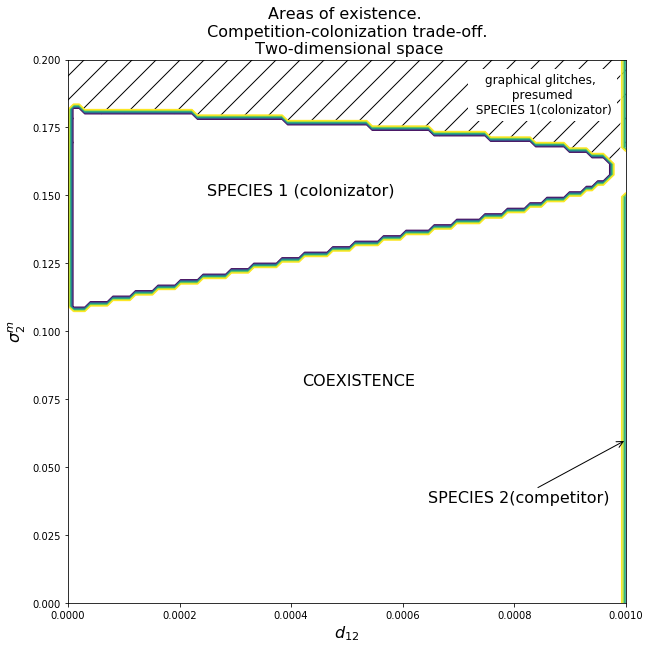
\includegraphics[width=.95\linewidth]{arccto08d2.png}
  \caption{Areas of coexistence in described parameter space}
  \label{fig:cctod2:sub2}
\end{subfigure}
\caption{Realization of Competition-Colonization Trade-Off mechanims in $\sigma^m_2$ and $d'_{12}$ parameter space in case of \emph{two-dimensional habitat}. Other parameters are chosen as follows:  $b_{1}=b_{2}=0.4
		, d_{1}=d_{2}=0.2
		, d'_{11}=d'_{22}=d'_{21}=0.001,
		\sigma_{1}^{m}=0.04
            , \sigma_{11}^{w}=\sigma_{12}^{w}=\sigma_{21}^{w}=\sigma_{22}^{w}=0.04$}
\label{fig:cctod2}
\end{figure*}


\begin{figure*}
\centering
\begin{subfigure}{.5\textwidth}
  \centering
  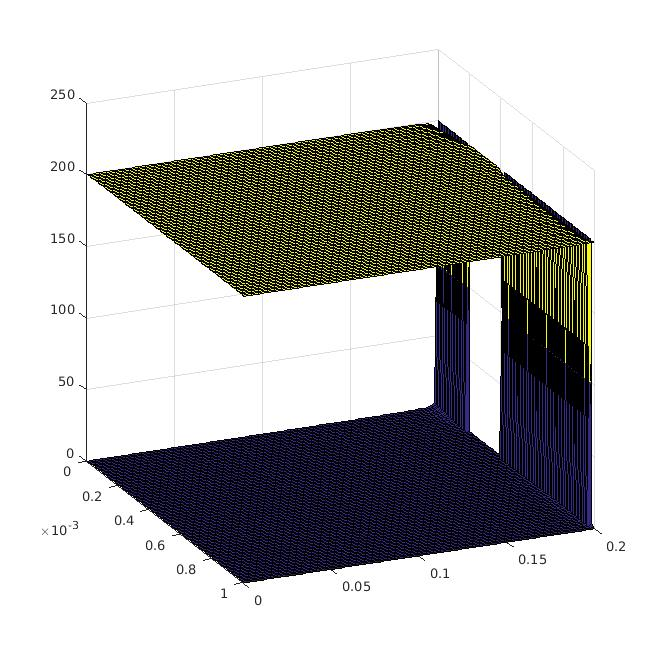
\includegraphics[width=.95\linewidth]{N1N2cctoD3.jpg}
  \caption{Surfaces of first moment \(N_1\) and \(N_2\) in described parameter space}
  \label{fig:cctod3:sub1}
\end{subfigure}%
\begin{subfigure}{.5\textwidth}
  \centering
  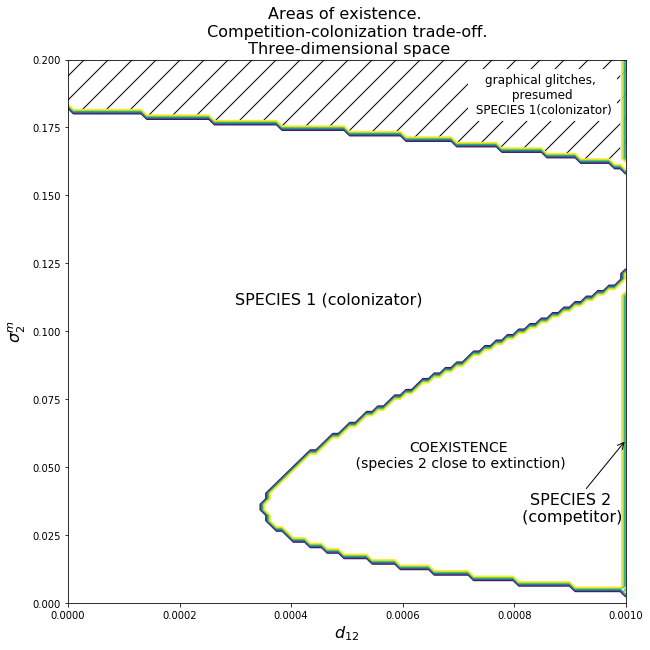
\includegraphics[width=.95\linewidth]{arccto08d3.png}
  \caption{Areas of coexistence in described parameter space}
  \label{fig:cctod3:sub2}
\end{subfigure}
\caption{Realization of Competition-Colonization Trade-Off mechanisms in $\sigma^m_2$ and $d'_{12}$ parameter space in case of \emph{three-dimensional habitat}. Other parameters are chosen as follows:  $b_{1}=b_{2}=0.4
		, d_{1}=d_{2}=0.2
		, d'_{11}=d'_{22}=d'_{21}=0.001,
		\sigma_{1}^{m}=0.04
            , \sigma_{11}^{w}=\sigma_{12}^{w}=\sigma_{21}^{w}=\sigma_{22}^{w}=0.04$}
\label{fig:cctod3}
\end{figure*}


\begin{itemize}
    \item an intreval chosen for \(d'_{12}\) should be enlarged in order to obtain greater area of competitor existence;
    \item the general concept of competition-colonization trade-off holds in all three dimensions; although it should be pointed out that the mechanisms should not be treated as ''in order to make species coexist, make one of them overdispersed''; as shown by our figures increase of \( \sigma^m_2 \) leads to colonizator domination;
    \item as the dimensionality of the habitat rises, species-colonizator starts to expel species-competitor: it can be observed that area of the first species enlarges, area of species 2 shrinks and coexistence area moves (two-dimensional case) and shrinks (three-dimensional case);
    \item in three-dimensional case species 1 practically expels second one; we still can obtain coexistence area, but it should be taken into consideration that in this area density of species 2 is pretty close to 0; in the same time on the right edge of the space this density sharply rises to the state where competitor wins;
    \item as you may see on figures \ref{fig:cctod2:sub2} and \ref{fig:cctod3:sub2} that developed numerical method still has number of graphical glitches that are not clearly seen of surfaces' plots; this glitches are supposed to be handled by increasing numerical methods accuracy.
\end{itemize}

\subsection{Heteromyopia}

Here we put our current results for coexistence mechanism called heteromyopia which was proposed in [Murell et al. 2003]. The general principle is that coexistence can be caused in case when interspecies competition radius is larger that intraspecies one. In our model we found this phenomena in space $\left[ \sigma^w_{ii}; \sigma^w_{ij} \right] $ which are supposed to be equal (or close to equal).

We focus our research on effects of dimensionality for the described mechanism. Figures \ref{fig:hmd1}, \ref{fig:hmd2} and \ref{fig:hmd3} are devoted to $\mathbb{R}^1$, $\mathbb{R}^2$ and $\mathbb{R}^3$ respectively. We propose new improved method with fewer mistakes for two-dimensional
case and utterly new method for three-dimensional case. For each case we put two subfigures: surfaces of species densities for each pair \( (\sigma^w_{ii}; \sigma^w_{ij}) \) and areas in the parameter space that support co-existence or existence of only one species which is denoted by its number on the picture.

We stress out following things regarding obtained results and its further analysis:

\begin{figure*}[ht]
	\centering
	\begin{subfigure}{.5\textwidth}
		\centering
		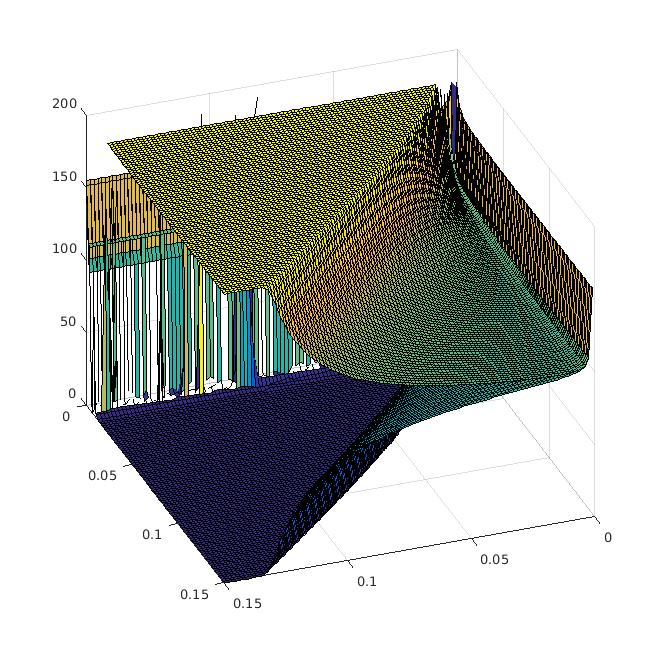
\includegraphics[width=.93\linewidth]{N1N2hm08D1.jpg}
		\caption{Surfaces of first moment \(N_1\) and \(N_2\) in described parameter space}
		\label{fig:hmd1:sub1}
	\end{subfigure}%
	\begin{subfigure}{.5\textwidth}
		\centering
		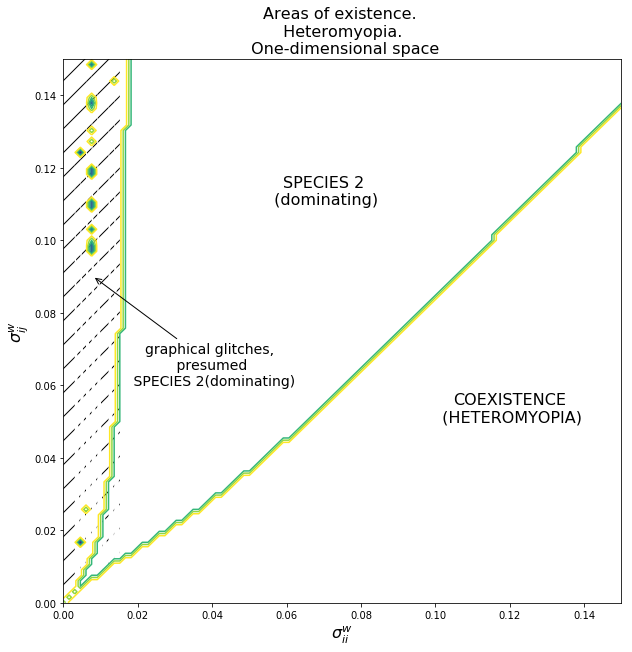
\includegraphics[width=.93\linewidth]{arhm08d1.png}
		\caption{Areas of coexistence in described parameter space} 
		\label{fig:hmd1:sub2}
	\end{subfigure}
	\caption{Realization of Heteromyopia mechanisms in  $\sigma_{11}^{w}=\sigma_{22}^{w}$ and $\sigma_{12}^{w}=\sigma_{21}^{w}$ parameter space in case of \emph{one-dimensional habitat}. Other parameters are chosen as follows: $b_{1}=b_{2}=0.4
		, d_{1}=d_{2}=0.2
		, d'_{11}=d'_{22}=d'_{21}=d'_{12}=0.001,
		\sigma_{1}^{m}=\sigma_{2}^{m}=0.06$. }
	\label{fig:hmd1}
\end{figure*}
\begin{figure*}[ht]
	\centering
	\begin{subfigure}{.5\textwidth}
		\centering
		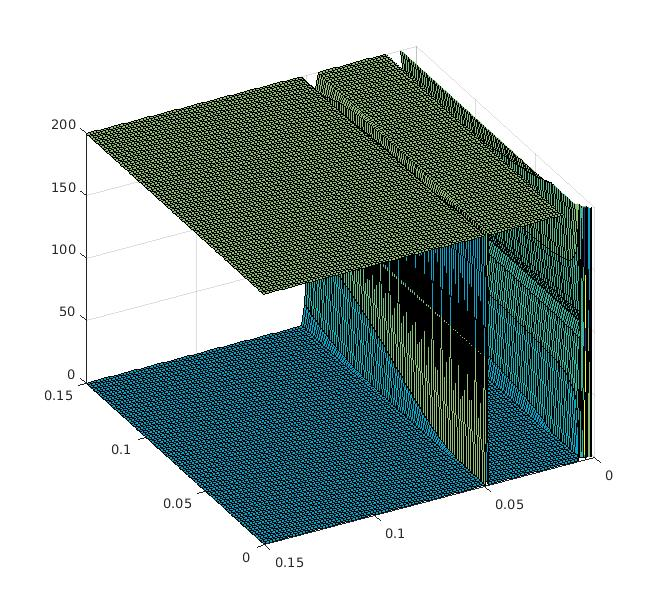
\includegraphics[width=.93\linewidth]{N1N2hm04D2.jpg}
		\caption{Surfaces of first moment \(N_1\) and \(N_2\) in described parameter space}
		\label{fig:hmd2:sub1}
	\end{subfigure}%
	\begin{subfigure}{.5\textwidth}
		\centering
		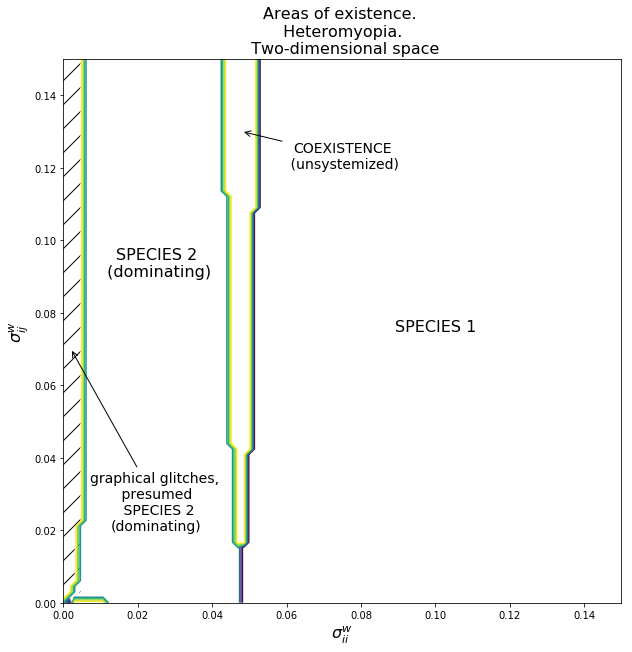
\includegraphics[width=.93\linewidth]{arhm08d2.png}
		\caption{Areas of coexistence in described parameter space}
		\label{fig:hmd2:sub2}
	\end{subfigure}
	\caption{Realization of Heteromyopia mechanisms in  $\sigma_{11}^{w}=\sigma_{22}^{w}$ and $\sigma_{12}^{w}=\sigma_{21}^{w}$ parameter space in case of \emph{two-dimensional habitat}. Other parameters are chosen as follows: $b_{1}=b_{2}=0.4
		, d_{1}=d_{2}=0.2
		, d'_{11}=d'_{22}=d'_{21}=d'_{12}=0.001,
		\sigma_{1}^{m}=\sigma_{2}^{m}=0.06$. }
	\label{fig:hmd2}
\end{figure*}
\begin{figure*}[ht]
	\centering
	\begin{subfigure}{.5\textwidth}
		\centering
		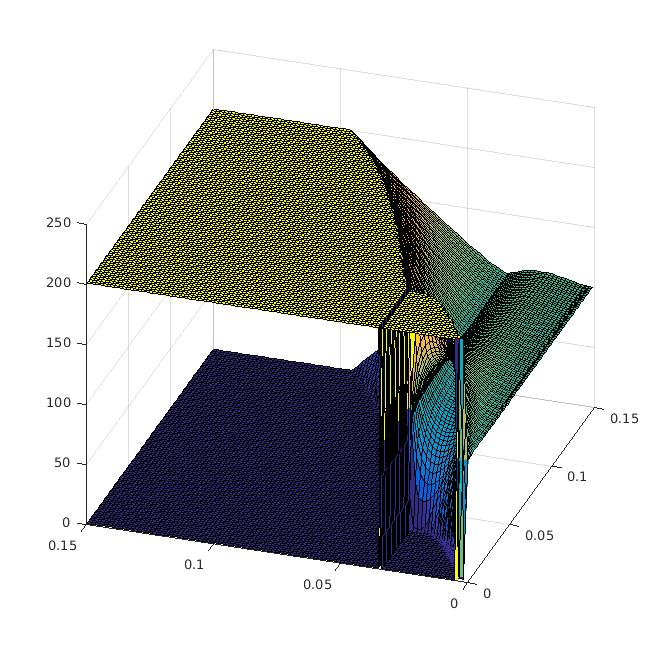
\includegraphics[width=.93\linewidth]{N1N2hm08D3.jpg}
		\caption{Surfaces of first moment \(N_1\) and \(N_2\) in described parameter space}
		\label{fig:hmd3:sub1}
	\end{subfigure}%
	\begin{subfigure}{.5\textwidth}
		\centering
		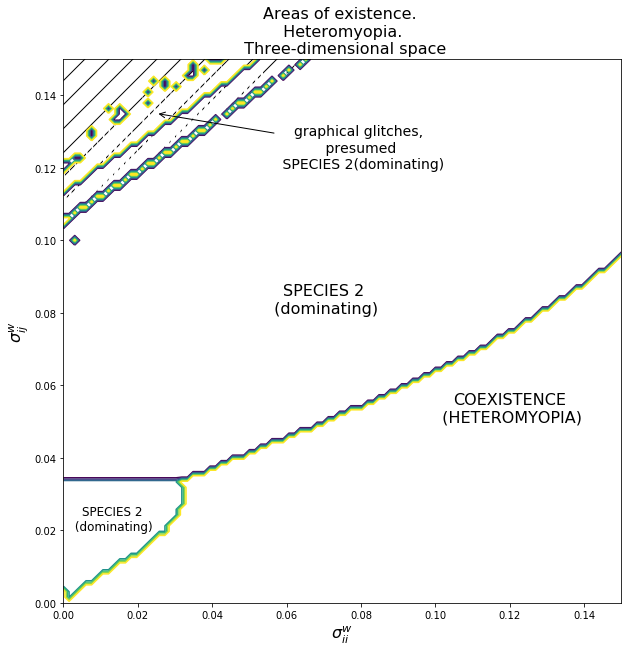
\includegraphics[width=.93\linewidth]{arhm08d3.png}
		\caption{Areas of coexistence in described parameter space}
		\label{fig:hmd3:sub2}
	\end{subfigure}
	\caption{Realization of Heteromyopia mechanisms in  $\sigma_{11}^{w}=\sigma_{22}^{w}$ and $\sigma_{12}^{w}=\sigma_{21}^{w}$ parameter space in case of \emph{three-dimensional habitat}. Other parameters are chosen as follows: $b_{1}=b_{2}=0.4
		, d_{1}=d_{2}=0.2
		, d'_{11}=d'_{22}=d'_{21}=d'_{12}=0.001,
		\sigma_{1}^{m}=\sigma_{2}^{m}=0.06$. }
	\label{fig:hmd3}
\end{figure*}


\begin{itemize}
	\item the general concept of the heteromyopia mechanism has been found in one- and three-dimensional cases only; 
	in both cases it is not exactly condition of strict inequality which was proposed in [Murrell et al. 2003] for coexistence arises, but linear approximation is still can be treated as a good call; 
	\item two-dimensional case does not included any pattern similar to heteromyopia that seems to be rather dissapointing;
	\item as you may see on figures \ref{fig:hmd1:sub2}, \ref{fig:hmd2:sub2} and \ref{fig:hmd3:sub2} that developed numerical method, as on aforementioned pictures for competition-colonization trade-off, has number of graphical glitches; this glitches are supposed to be handled by increasing numerical methods accuracy.
\end{itemize}


\newpage

\appendix

\section{System of equations}

\label{sec:appA}

Assume the problem stated earlier as follows:
\[
\forall i,j: \; \frac{\partial N_i(t)}{\partial t}=0, \;\; \frac{\partial C_{ij}(\vec{\xi}, t)}{\partial t}=0.
\]
System's dynamic equations:
\begin{eqnarray*}
	\frac{d}{dt}N_{i}=(b_{i}-d_{i})N_{i}-\sum_{j}\int_{\mathbb{R}^{n}}w_{ij}(\xi)C_{ij}(\xi)d\xi
\end{eqnarray*}
\begin{eqnarray*}
	\frac{d}{dt}C_{ij}(\xi)= \delta_{ij}m_{i}(-\xi)N_{i}+\int_{\mathbb{\mathbb{R}}^{n}}m_{i}(\xi')C_{ij}(\xi+\xi')d\xi'-\\
	-d_{i}C_{ij}(\xi)-\sum_{k}\int_{\mathbb{\mathbb{R}}^{n}}w_{ik}(\xi')T_{ijk}(\xi,\xi')d\xi-w_{ij}(\xi)C_{ij}(\xi)+\\+\langle i,j,\xi\to j,i,-\xi\rangle
\end{eqnarray*}

We propose denotations such as $[f*g](\xi)=\int_{\mathbb{\mathbb{R}}^{n}}f(\xi')g(\xi'+\xi)d\xi'$
as classic \emph{convolution }and $y_{ij}=\int_{\mathbb{\mathbb{R}}^{n}}w_{ij}(\xi')C_{ij}(\xi')d\xi'$.
Also we use normalized moments $C_{ij}=\frac{C_{ij}}{N_{i}N_{j}}$
and $T_{ijk}=\frac{T_{ijk}}{N_{i}N_{j}N_{k}}$ and centralized $D_{ij}(\xi)=C_{ij}(\xi)-1$.

All arising equations should be closed considering:

\begin{multline*}
T_{ijk}(\xi,\xi') = \frac{\alpha}{2}\left(\frac{C_{ij}(\xi)C_{ik}(\xi')}{N_{i}}+\frac{C_{ij}(\xi)C_{jk}(\xi'-\xi)}{N_{j}}+\right.\\
\left.+\frac{C_{ik}(\xi')C_{jk}(\xi'-\xi)}{N_{k}}-1\right)+(1-\alpha)\frac{C_{ij}(\xi)C_{ik}(\xi')}{N_{i}}
\end{multline*}
with $\alpha=\frac 2 5$.

Here we put resulting system:

\begin{eqnarray*}
	N_{1}=\frac{(b_{1}-d_{1})y_{22}-(b_{2}-d_{2})y_{12}}{y_{11}y_{22}-y_{12}y_{21}}
	\\
	N_{2}=\frac{(b_{2}-d_{2})y_{11}-(b_{1}-d_{1})y_{21}}{y_{11}y_{22}-y_{12}y_{21}}
\end{eqnarray*}
\begin{widetext}
	\begin{multline*}
	((1-\frac{\alpha}{2})b_{1}+\frac{\alpha}{2}(d_{1}+N_{1}d'_{11}+N_{2}d'_{12})+w_{11})D_{11}=\frac{m_{1}}{N_{1}}+\left[m_{1}*D_{11}\right]-w_{11}-\\
	-\frac{\alpha}{2}N_{1}((D_{11}+2)[w_{11}*D_{11}]+[w_{11}D_{11}*D_{11}])-\\
	-\frac{\alpha}{2}N_{2}((D_{11}+2)[w_{12}*D_{12}]+[w_{12}D_{12}*D_{12}])
	\end{multline*}

	\begin{multline*}
	((1-\frac{\alpha}{2})b_{2}+\frac{\alpha}{2}(d_{2}+N_{1}d'_{21}+N_{2}d'_{22})+w_{22})D_{22}=\frac{m_{2}}{N_{2}}+\left[m_{2}*D_{22}\right]-w_{22}-\\
	-\frac{\alpha}{2}N_{2}((D_{22}+2)[w_{22}*D_{22}]+[w_{22}D_{22}*D_{22}])-\\
	-\frac{\alpha}{2}N_{1}((D_{22}+2)[w_{21}*D_{12}]+[w_{21}D_{12}*D_{12}])
	\end{multline*}

	\begin{eqnarray*}
		((1-\frac{\alpha}{2})(b_{1}+b_{2})+\frac{\alpha}{2}(d_{1}+d_{2}+d'_{11}N_{1}+d'_{12}N_{2}+d'_{21}N_{1}+d'_{22}N_{2})+w_{12}+w_{21})D_{12}=\\{}
		[(m_{1}+m_{2})*D_{12}]-w_{12}-w_{21}-\\
		-\frac{\alpha}{2}N_{1}((D_{12}+2)([w_{11}*D_{12}]+[w_{21}*D_{11}])+[w_{21}D_{12}*D_{11}]+[w_{11}D_{11}*D_{12}])-\\
		-\frac{\alpha}{2}N_{2}((D_{12}+2)([w_{12}*D_{22}]+[w_{22}*D_{12}])+[w_{22}D_{22}*D_{12}]+[w_{12}D_{12}*D_{22}])
	\end{eqnarray*}
\end{widetext}

\section{Heuristics for two- and three-dimensional cases}

\label{sec:appB}

\subsection{Two-dimensional case}
By using ordinary Convolution theorem for $\mathbb{R}^2$:
\[[f**g]_{\mathbb{R}^2}=\hat{F}[F[f]\cdot F[g]]\]
Assume spherical transform:
\begin{multline*}
F[f](\omega_x, \omega_y)=\int\limits_{-\infty}^{+\infty}\int\limits_{-\infty}^{+\infty}f(x,y)e^{-i(\omega_x x+\omega_y y)}dxdxy=\\
=\int\limits_{0}^{+\infty}\int\limits_{-\pi}^{\pi}f(r,\theta)e^{-ir\rho\cos(\psi-\theta)}rdrd\theta.
\end{multline*}
By radial symmetry we obtain:
\[
F[f](\rho,\psi)=\int\limits_{0}^{+\infty}rf(r)dr\int\limits_{-\pi}^{\pi}e^{-ir\rho\cos(\psi-\theta)}d\theta
\]
\[
F[f](\rho,\psi)=2\pi\int\limits_{0}^{+\infty}rf(r)J_0(r\rho )dr,
\]
which is known as Hankell transfrom of the 0-order, where $
J_0(x)=\frac{1}{2\pi}\int\limits_{-\pi}^{\pi}e^{-ix\cos\tau}d\tau$ --- Bessel function of 0-order and quasi-Convolution theorem can be formulated:
\[
H[f*g]=H[(2\pi)^2 H[f] \cdot H[g]]
\]
with the same numerical complexity as $[f*g]$.

\subsection{Three-dimensional case}

By using ordinary Convolution theorem for $\mathbb{R}^3$:
\[[f***g]_{\mathbb{R}^3}=\hat{F}[F[f]\cdot F[g]]\]
Treat $F[f]$ as in complex form:
$$
F[f]=\int\limits_{\mathbb{R}^3}f(\vec{x})e^{-i(\vec{w},\vec{x})}d\vec{x}
$$
Assume spherical transform 
$$
F[f]=\int_0^{+\infty}\int_0^{2\pi}\int_{-\pi/2}^{\pi/2}f(r, \phi, \psi)e^{-i(\vec{w},\vec{x})}r^2\sin \psi d\phi d\psi dr
$$
By applying Laplass problem on a sphere we obtain the set of orthogonal solutions:
$$
	y(\phi, \psi)=C_1\cdot P(\cos \phi )e^{iC_2 \psi}
$$
where $P(x)$ --- Legendre polynome, $C_1$ and $C_2$ are constants dependent on order of $P(x)$. Thus we may obtain a spherical harmonics series for $e^{iC_2\psi}$ which can be merged into Fourier transform giving after simplification:
\[
[f***g]=4\pi[f*g]
\]
with the same numerical complexity as [f*g]. 

Proposed heuristics are only applicable for radially symmetric case. It should be pointed out that this by far proves that this characteristic is invariant for iterative operator used for describing equilibrium points thus we cannot leave a space of radially symmetric functions.

Also we'd like to put that only after proposed heuristics the task of mechanism testing if thorough parameter spaces turned into solvable in reasonable time. In words, coming up with this Appendix was a necessity.

% If in two-column mode, this environment will change to single-column format so that long equations can be displayed. 
% Use only when necessary.
%\begin{widetext}
%$$\mbox{put long equation here}$$
%\end{widetext}

% Figures should be put into the text as floats. 
% Use the graphics or graphicx packages (distributed with LaTeX2e).
% See the LaTeX Graphics Companion by Michel Goosens, Sebastian Rahtz, and Frank Mittelbach for examples. 
%
% Here is an example of the general form of a figure:
% Fill in the caption in the braces of the \caption{} command. 
% Put the label that you will use with \ref{} command in the braces of the \label{} command.
%
% \begin{figure}
% \includegraphics{}%
% \caption{\label{}}%
% \end{figure}

% Tables may be be put in the text as floats.
% Here is an example of the general form of a table:
% Fill in the caption in the braces of the \caption{} command. Put the label
% that you will use with \ref{} command in the braces of the \label{} command.
% Insert the column specifiers (l, r, c, d, etc.) in the empty braces of the
% \begin{tabular}{} command.
%
% \begin{table}
% \caption{\label{} }
% \begin{tabular}{}
% \end{tabular}
% \end{table}




% If you have acknowledgments, this puts in the proper section head.
%\begin{acknowledgments}
% Put your acknowledgments here.
%\end{acknowledgments}

% Create the reference section using BibTeX:
%\bibliography{your-bib-file}

\end{document}
%
% ****** End of file aiptemplate.tex ******
